\subsection{Evaluation}
\label{sec:eval}

\begin{figure}[!t]
  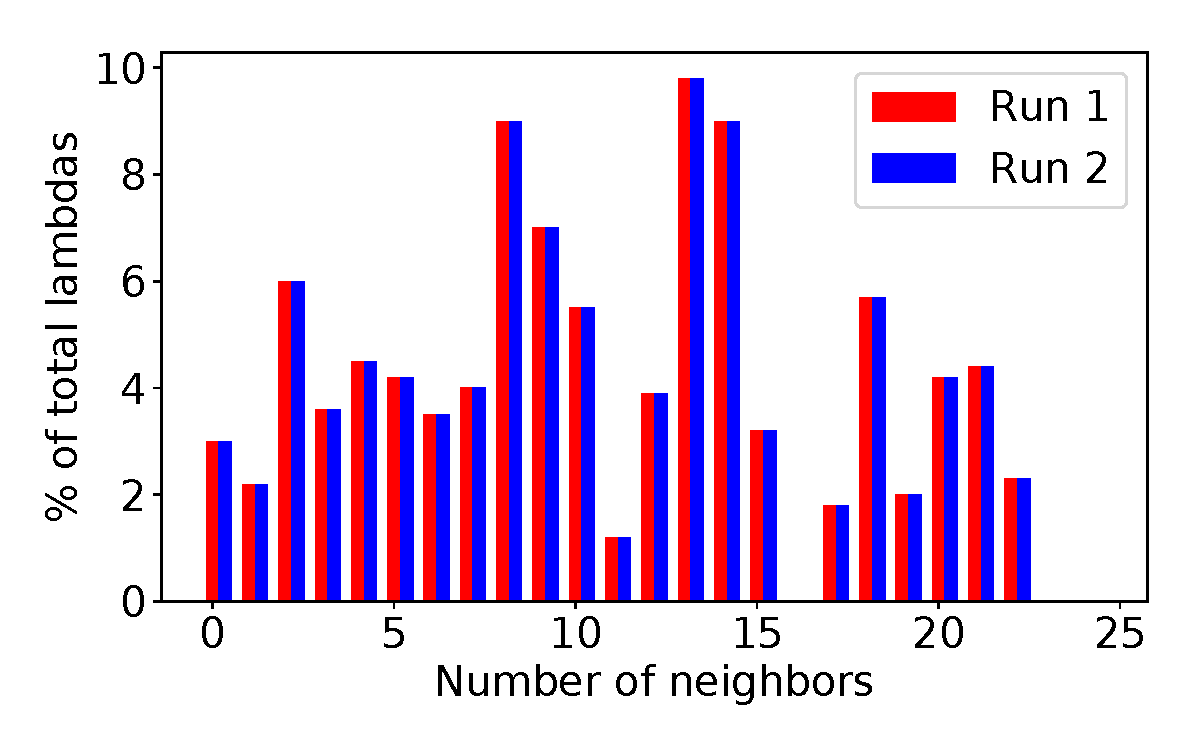
\includegraphics[width=.99\linewidth]{fig/correlation.pdf}
  \caption{This figure shows the fraction of lambdas by the number of neighbors 
  they identify for two independent runs that use same set of underlying AWS
  containers. The perfect correlation shows that both runs depict the co-residence 
  status of those containers regardless of the lambdas that ran on them, providing
  evidence for the correctness of our approach.
\label{fig:correlation}}
\end{figure}

% In this section, we evaluate the effectiveness of both our co-residence detection
% technique and our covert channel.
% \subsection{Co-residence Detector}

We next examine our co-residence detector with respect to reliability,
scalability, and speed, the desirable detection properties mentioned in
section~\ref{sec:methodology}.  We run all of our experiments with AWS
lambdas~\cite{awscloud}. Though we decide to focus on only one of the cloud
providers as a case study, we have previously shown in
section~\ref{sec:methodology} that this covert channel exists on the other
clouds, and thus we believe these experiments can be replicated on their serverless
functions as well. We use the C++ runtime in AWS lambdas as it allows pointer
arthmetic that is required to access the covert channel.

\subsubsection{Setup}
\label{subsec:expsetup}
We start by deploying a series of lambdas from an AWS lambda account.  Once
deployed, each lambda participates in the first phase of the protocol as noted
in section~\ref{sec:protocol:complexity}, thereby learning the largest ID of
their neighbors. As bit-flip errors are possible, we repeat the same phase for
two more (independent) "rounds" and take the majority result to record the ID
seen by this lambda.  If all three rounds result in different IDs, we classify
this lambda as erroneous and report it in the error rate. We group all the
lambdas that saw the same ID as successful and neighbors. We repeat the
experiments for different lambda sizes and in various cloud regions.

\subsubsection{Reliability}
We consider the results of the technique reliable when most of the deployed
lambdas successfully see the same result in a majority of the independent rounds
(indicating lesser bit-flip errors) and the resulting co-resident groups we
see examine the ground truth.  For the former requirement, 
we ran an experiment with 1000 AWS
lambdas and compared the error rate across different lambda sizes (the error
rate indicates the fraction of these 1000 lambdas that returned erroneous result).
\amirian{the phrasing of majority here confuses me a bit but im not sure
how to fix it \anil{defined in above paragraph}} Figure~\ref{fig:errorrates} 
indicates that smaller lambdas exhibit
more errors.  This is expected because, as discussed in section
\ref{sec:method:noise}, these lambdas experience lossy communication, making it
harder for our technique to sense contention. Lambdas that are 1.5 GB and
larger, though, exhibit a 100\% success rate. Of these errors, false positives are 
rare as we run multiple independent rounds, and the chance of two rounds erring at 
the same bit(s) (to give the same wrong result across the majority of rounds) is low. 
False negatives, however, are common and contribute to most of the errors.

\textbf{Correctness} 
To determine correctness, we require ground truth on which lambdas are
co-resident with one another. While such information is not available, we are
able to ascertain correctness of our approach by utilizing an AWS caching
mechanism. On AWS, each lambda runs in a dedicated container (sandbox).  After
execution, AWS caches these containers in order to reuse
them~\cite{awscontainerreuse} and mitigate "cold start" latencies. 
We found that global objects like files persist across warm-starts,
and can be used to track all the lambdas that were
ever executed in a particular container. Using this insight, we are able to 
validate that
identical experiments repeated within minutes of one another will use the same
set of underlying containers for running the deployed lambdas. This allows us 
to test the correctness of our technique as variance in the co-residence 
results between these experiments would suggest a lack of fidelity in our approach. 
(Note that the warm-start information cannot be used to detect co-residency itself 
nor can it be used to verify correctness in all scenarios.)


\begin{figure}[!t]
  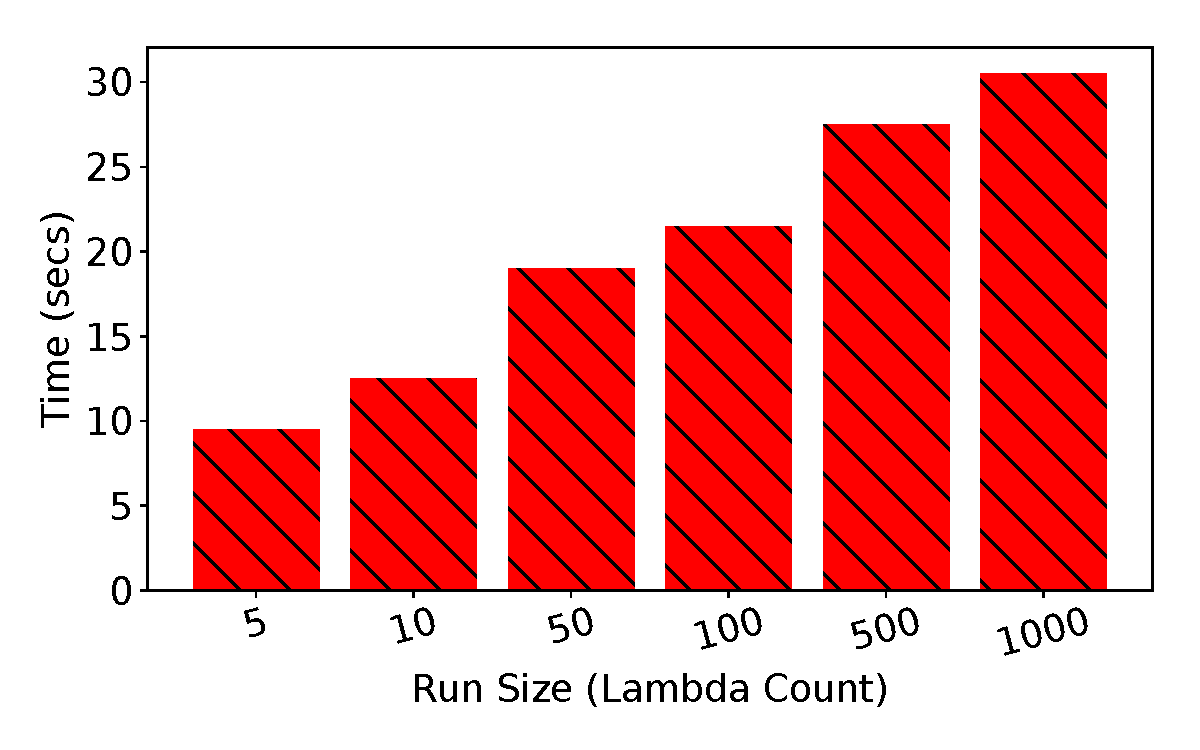
\includegraphics[width=.99\linewidth]{fig/runtimes.pdf}
  \caption{We present the average execution time of the lambdas for co-resident
  runs with a varying number of lambdas. The execution time increases
  logarithmically with the number of lambdas demonstrating the scalability of
  co-residence detection with our technique.
\label{fig:runtimes}}
\end{figure}


\begin{figure}[!t]
  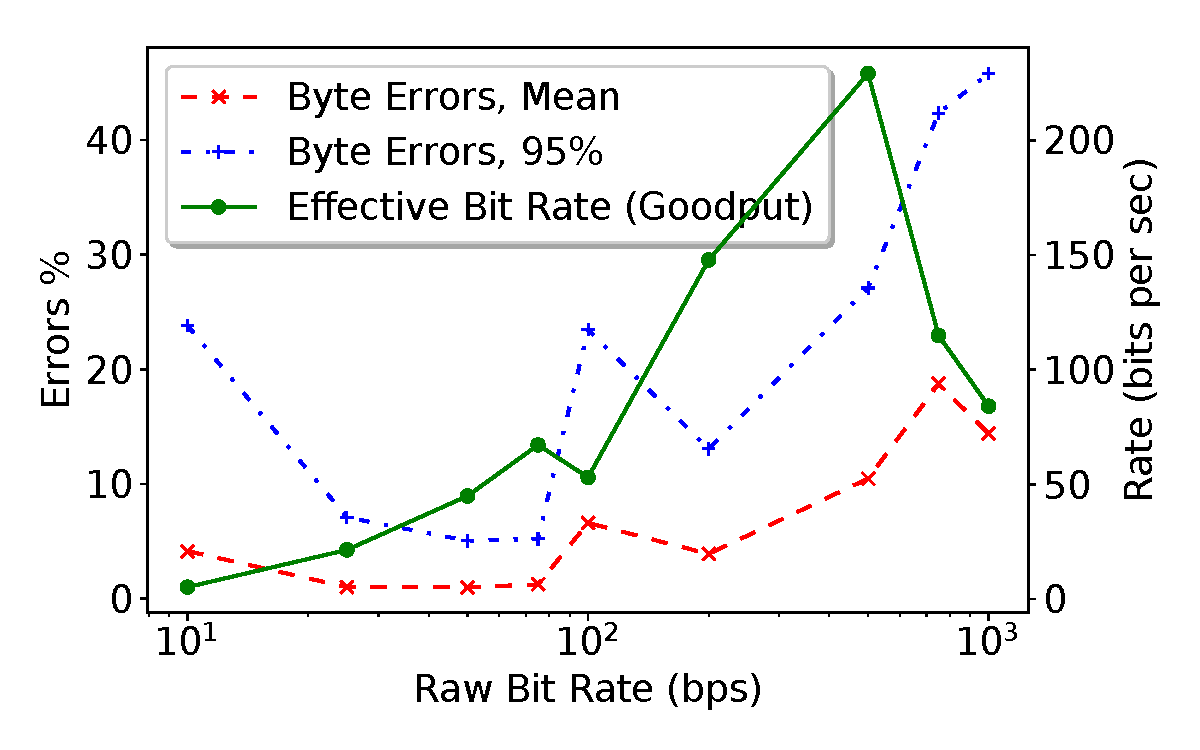
\includegraphics[width=.99\linewidth]{fig/channel_rate_3gb.pdf}
 \caption{The dashed lines in the figure presents the mean error ratio at 50\% and 95\%
 confidence when sending bits at various rates over the covert channel. The solid 
 line shows the effective channel rate after accounting for the overhead of 
 error correction at the 95\% error.
\label{fig:channel}}
\end{figure}

% Figures from the next section
% Moved here for formatting

\begin{figure*}[!t]
  \begin{subfigure}{.33\textwidth}
    \centering
    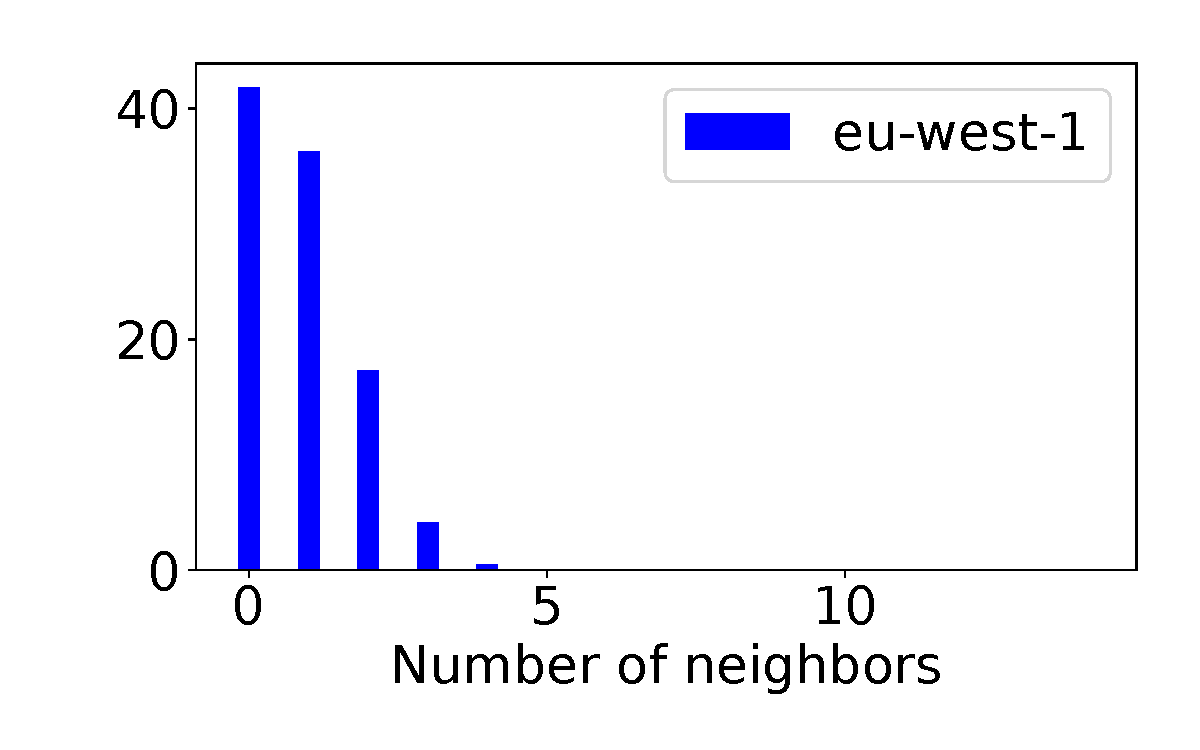
\includegraphics[width=.99\linewidth]{fig/colocation-eu-west-1.pdf}
  %   \caption{1a}
  %   \label{fig:sfig1}
  \end{subfigure}%
  \begin{subfigure}{.33\textwidth}
    \centering
    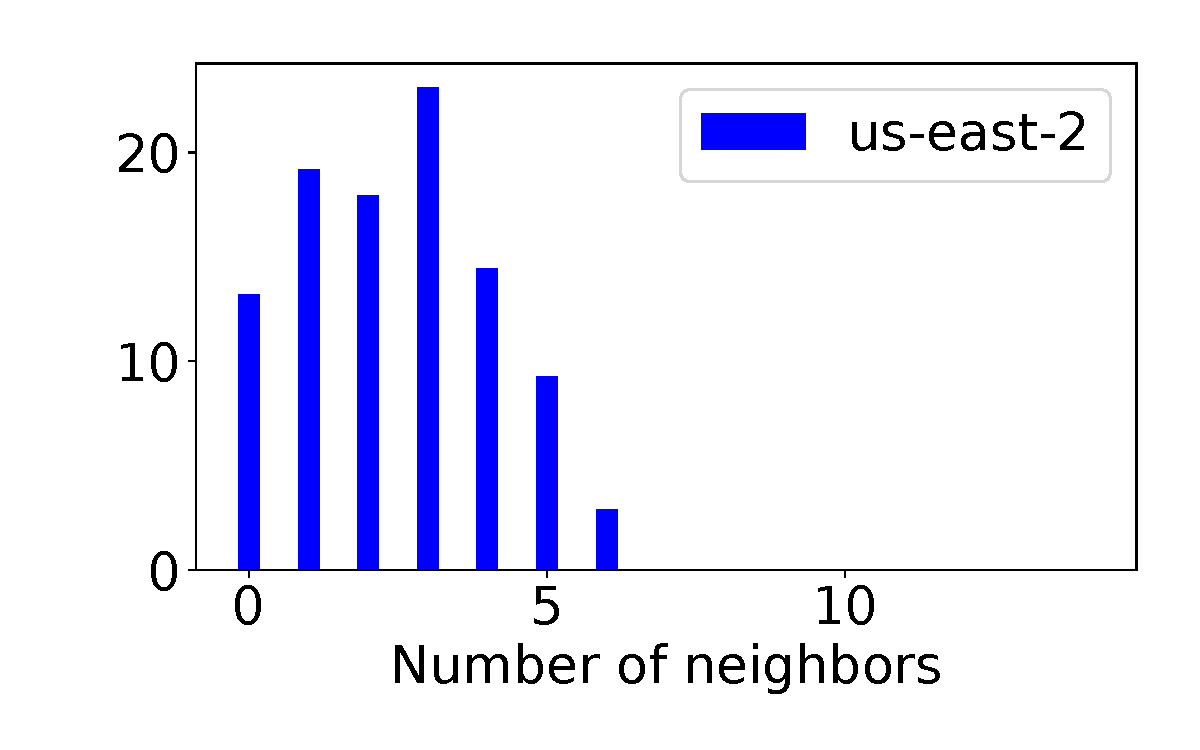
\includegraphics[width=.99\linewidth]{fig/colocation-us-east-2.pdf}
  %   \caption{1b}
  %   \label{fig:sfig2}
  \end{subfigure}
  \begin{subfigure}{.33\textwidth}
    \centering
    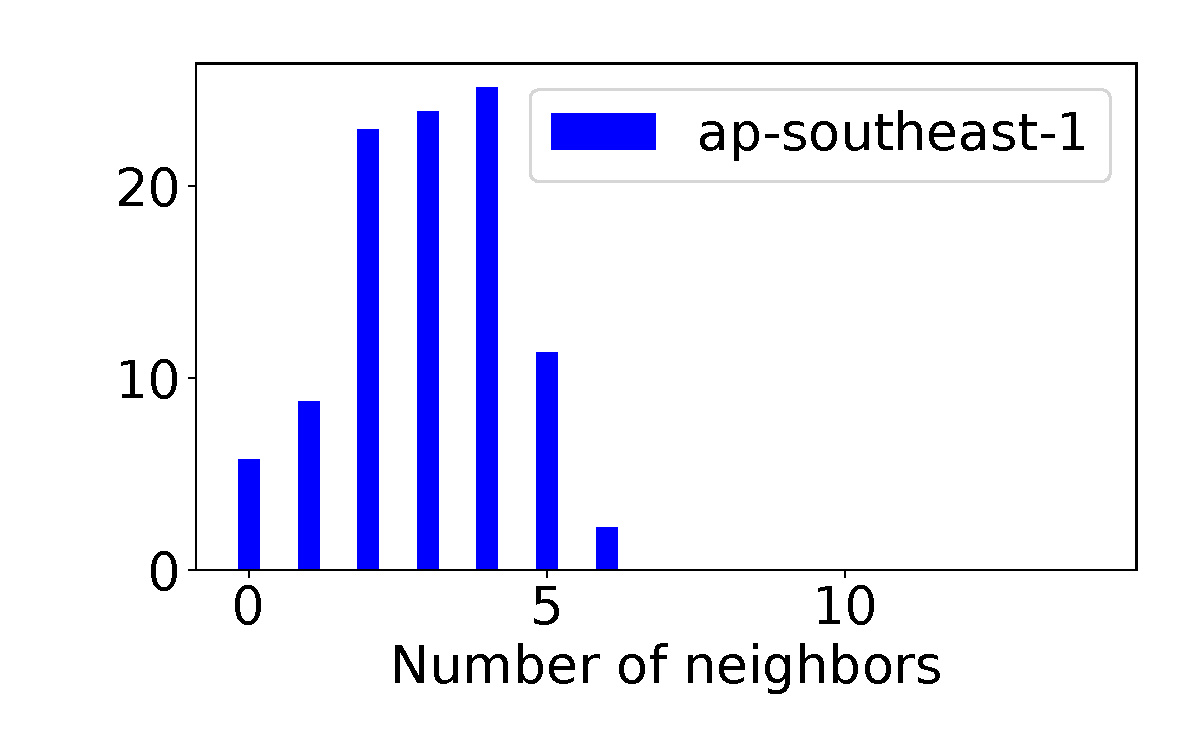
\includegraphics[width=.99\linewidth]{fig/colocation-ap-southeast-1.pdf}
  %   \caption{1b}
  %   \label{fig:sfig2}
  \end{subfigure}
  
  \begin{subfigure}{.33\textwidth}
    \centering
    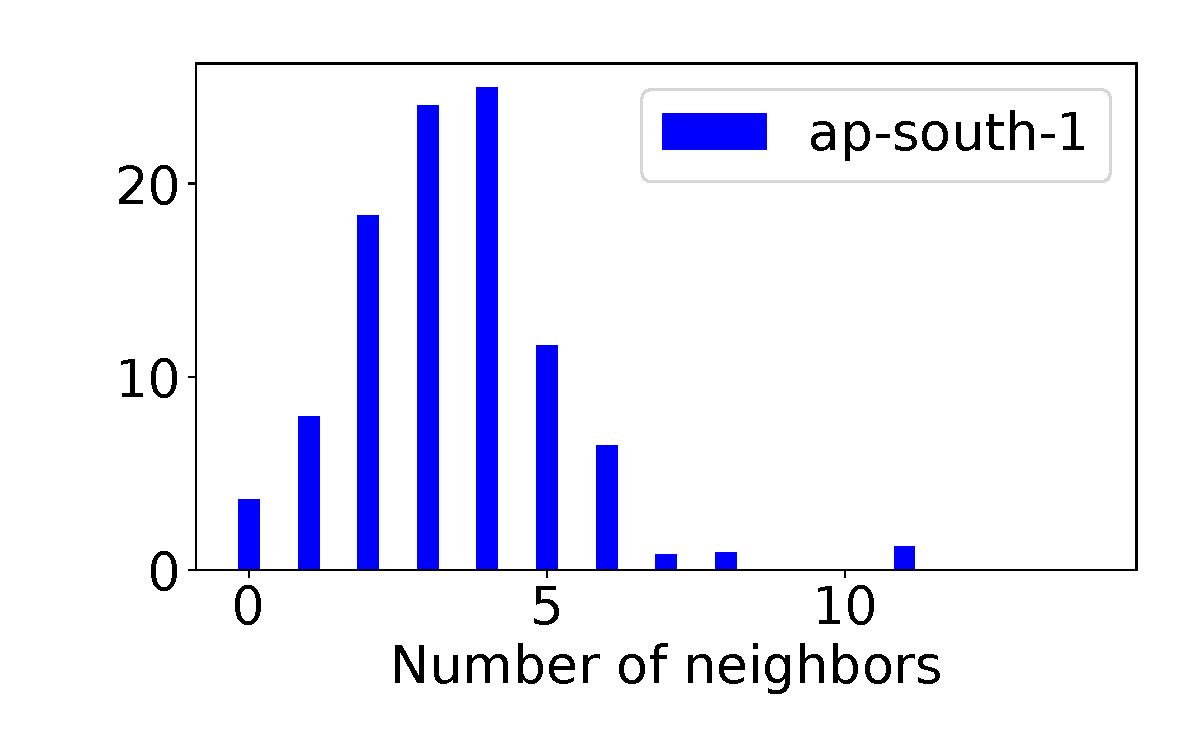
\includegraphics[width=.99\linewidth]{fig/colocation-ap-south-1.pdf}
  %   \caption{1a}
  %   \label{fig:sfig1}
  \end{subfigure}%
  \begin{subfigure}{.33\textwidth}
    \centering
    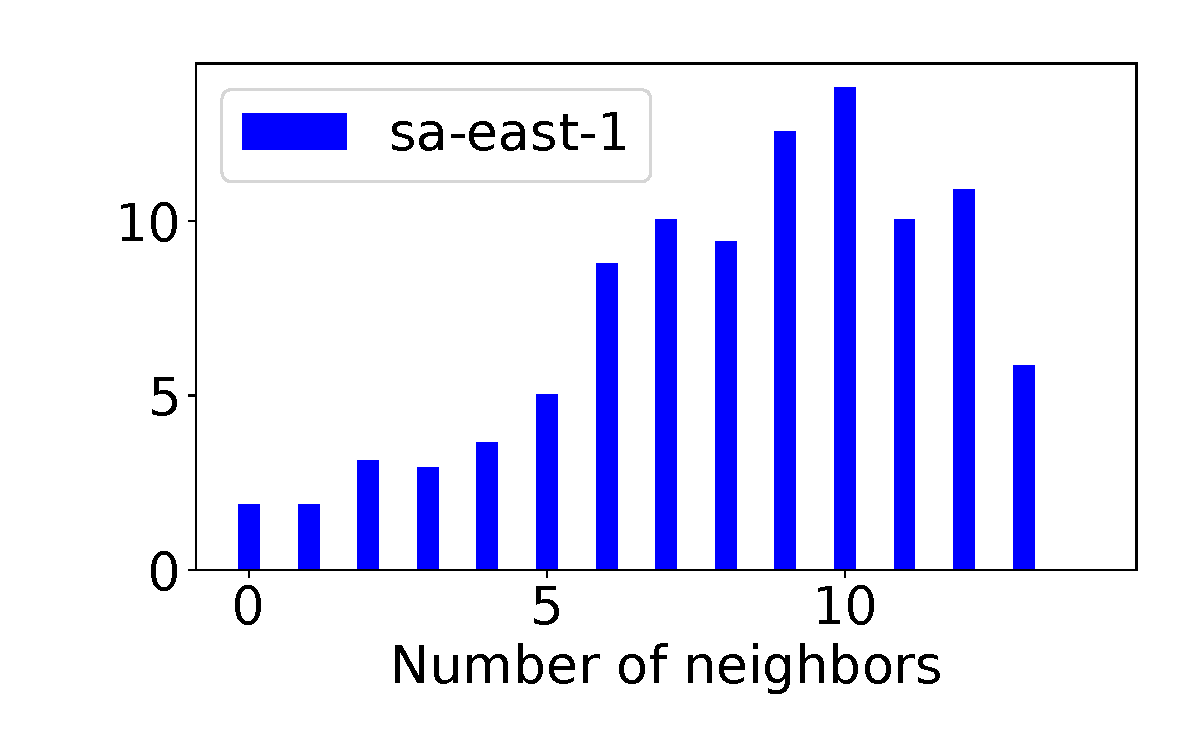
\includegraphics[width=.99\linewidth]{fig/colocation-sa-east-1.pdf}
  %   \caption{1b}
  %   \label{fig:sfig2}
  \end{subfigure}
  \begin{subfigure}{.33\textwidth}
    \centering
    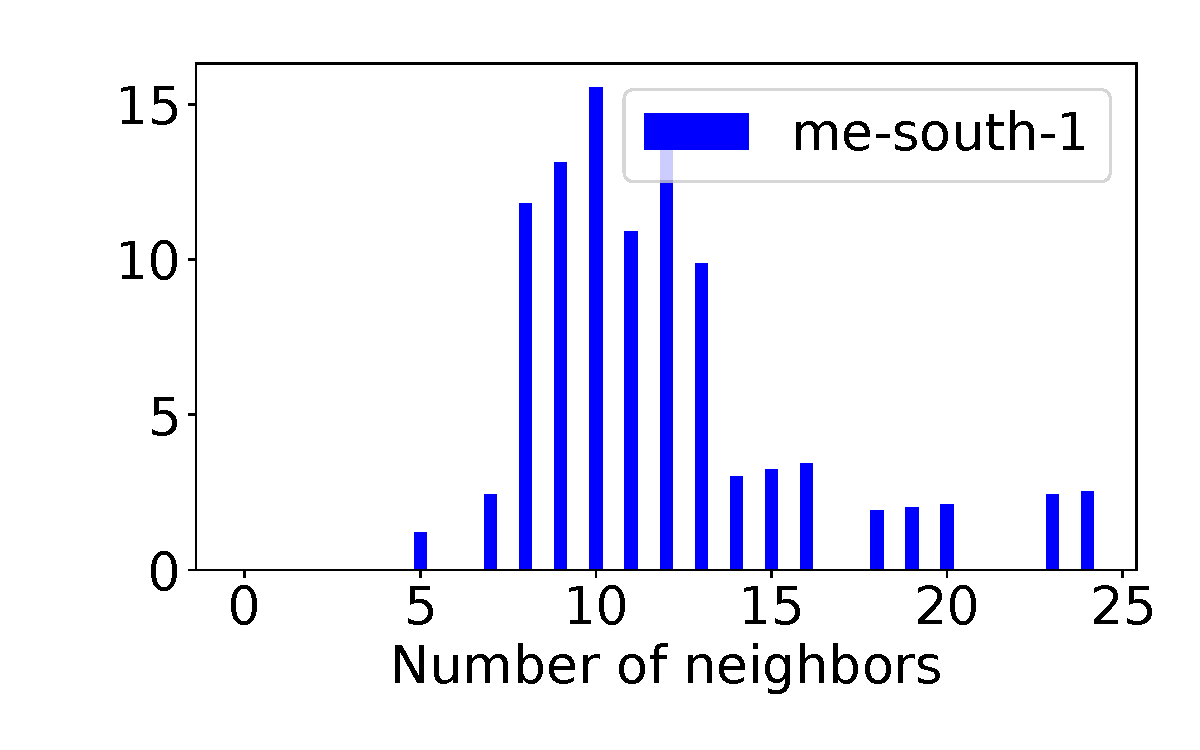
\includegraphics[width=.99\linewidth]{fig/colocation-me-south-1.pdf}
  %   \caption{1b}
  %   \label{fig:sfig2}
  \end{subfigure}
  \caption{We present co-residence results from a 1000-lambda run in different AWS regions. Each bar shows the fraction 
  of those 1000 lambdas (in \%) that discovered a certain number of neighbors. The total amount and density of co-residence 
  vary widely across regions, perhaps based on the size of those regions and the lambda activity within them. }
  \label{fig:awsregions}
  \end{figure*}

To demonstrate this correlation, we run an
experiment with 1000 1.5GB cold-started lambdas (ID'ed 1 to 1000) in one of
newer AWS regions (me-south-1), which resulted in many co-resident groups.
We repeat the experiment within a few seconds, thereby ensuring that all 1000
lambdas are warm-started on the second trial (i.e., they use the same set of
containers from the previous experiment).  For each co-resident group of lambdas
in the latter experiment, we observed that their predecessor lambdas (that used
the same set of containers) in the former experiment formed a co-resident group
as well. That is, while the lambdas to the underlying container mapping is
different across both experiments, the results of the experiments agree
perfectly on the container colocation. Figure~\ref{fig:correlation} shows that
both experiments saw the same number of co-resident groups of different sizes,
showing the correctness of the results of our mechansim.

\subsubsection{Scalability \& Speed}
\label{sec:eval:scalability}
One of the key properties of this technique is its short execution time and
scalability. Since communicating each binary bit of the ID takes one second, we
are able to scale the technique logarithmically with the number of lambdas
involved. Figure~\ref{fig:runtimes} shows this result with experiments
involving different number of lambdas. For example, in an experiment with 1000
lambdas, each lambda can find its neighbors within a minute of its invocation,
leaving ample time for the attacker to then establish the covert channel and use
it to send information (for reference, lambdas on AWS can only run for 15
minutes at most).  The logarithmic scale of our method also indicates that the
cost per lambda scales logarithmically, making neighbor detection
cost-effective.  For example, one 1000 lambda run with 1.5 GB lambdas cost
around just 1.5 USD. 

% mention cost of one run?


%\paragraph{Generality}
%\todo{We only implemented it on AWS. This requires us to implement it on 
%Azure and GCP, and report some results. \textbf{Needs considerable effort}}
